\documentclass[aps,pre,12pt,preprint,%
	onecolumn,showpacs,showkeys,nofootinbib]{revtex4-2}
%Chinese
	\usepackage[UTF8,fontset=fandol]{ctex}
%	\usepackage[datesep=/]{datetime2} % Use default
	\DeclareTextFontCommand{\textbf}{\sffamily}
%Presenting
	\usepackage[table]{xcolor}
	\usepackage{graphicx}
	\usepackage[font=small,format=plain,%
		labelfont=bf,textfont=it,%
		singlelinecheck=false]{caption}
	\usepackage[above]{placeins}
%	\usepackage{float} % Cause trouble for table footnotes
	\usepackage{wrapfig}
	\usepackage{tabularx,array,booktabs,multirow,bigstrut}
	\newcolumntype{C}[1]{>{\hsize=#1\hsize%
		\centering\arraybackslash}X}
	\newcommand{\minitab}[2][l]{%
		\begin{tabular}{#1}#2\end{tabular}}
	\usepackage{setspace,dcolumn}
	\usepackage{subfig}
	\usepackage{psfrag,epsfig}
%MathSetting
	\let\latexointop\ointop
	\usepackage{amsmath,bm,amssymb,esint,extarrows}
	\usepackage{upgreek,textcomp,mathrsfs}
	\usepackage[only,sslash]{stmaryrd}
	\usepackage{nicefrac,eqnarray}
%	\usepackage{amsthm} % Enable when necessary
%	\usepackage[mathscr]{eucal} % Enable when necessary
	\usepackage{mathtools,physics,siunitx}
	\usepackage{stackengine,varwidth}
	\usepackage{tikz}
	\usepackage{resizegather,empheq}
	\usetagform{default}
	\usepackage{calligra,fourier-orns}
	% Keep \oint unchanged by esint
	\let\ointop\undefined
	\let\ointop\latexointop
	% Define a scriptr 
	\DeclareMathAlphabet{\mathcalligra}{T1}{calligra}{m}{n}
	\DeclareFontShape{T1}{calligra}{m}{n}{<->s*[2.2]callig15}{}
	\newcommand{\scriptr}{\mathcalligra{r}\,}
	\newcommand{\rvector}{\pmb{\mathcalligra{r}}\,}
	% Useful shorthand
	\DeclarePairedDelimiter\ave{\langle}{\rangle}
	\newcommand\inlineeqno{\stepcounter{equation}\ (\theequation)}
	\newcommand{\sinc}{\operatorname{sinc}}
	\newcommand{\mbb}[1]{\mathbb{#1}}
	\newcommand{\mrm}[1]{\mathrm{#1}}
	\newcommand{\mcal}[1]{\mathcal{#1}}
	% Scaling and positioning
	\newcommand\scalemath[2]{\scalebox{#1}{\mbox{\ensuremath{\displaystyle #2}}}}
	\newcommand\raisemath[2]{\raisebox{#1\depth}{${#2}$}}
	\empheqset{box=\nicebox}
	% Presenting
	\newcommand*\nicebox[1]{\fbox{\hspace{1em}\addstackgap[5pt]{#1}\hspace{1em}}}

	\allowdisplaybreaks[2]
%ParagraphSetting
	\setlength{\parskip}{.3\baselineskip}
	\usepackage[defaultlines=2,all]{nowidow}
	\postdisplaypenalty=50
%PageSetting
	\usepackage{titlesec}
	\titleformat*{\section}{\large\bfseries}
	\usepackage[colorlinks=true,linkcolor=blue]{hyperref}
	\newcommand{\texstringonly}[1]{%
		\texorpdfstring{#1}{}}
	\usepackage[vmargin={3.5cm,4cm},hmargin=3cm,%
		footnotesep=\baselineskip]{geometry}
%	\usepackage[bottom]{footmisc} % Cause trouble for table footnotes
	\usepackage{changepage}
	% Autoref names
	\renewcommand{\tableautorefname}{\tablename}
	\renewcommand{\figureautorefname}{\figurename}
	% List settings
	\usepackage{enumitem}
	\setlist{itemsep=0pt,topsep=0pt,labelindent=\parindent,leftmargin=0pt,itemindent=*}
	% Some redefined lengths
	\setlength{\headsep}{1.6\baselineskip}
%	\setlength{\footnotesep}{3\parskip} % Use when necessary
	% Header
	\usepackage{fancyhdr,lastpage}
	\pagestyle{fancy}
%	\fancyhf{} % Clear default settings; disabled for now
	\cfoot{--\ \thepage\,/\,\pageref{LastPage} \ --}
	\setlength{\footskip}{2\baselineskip}
	\renewcommand{\headrulewidth}{0.1pt}
	\renewcommand{\headrule}{
		\ifnum\value{page}=1\relax\else
			\vbox to 2pt{
			\hbox to \headwidth{\dotfill}\vss}
		\fi}
	\fancypagestyle{titlepagestyle}{%
		\fancyhead{}
		\chead{
			\vspace{2.5\baselineskip}
			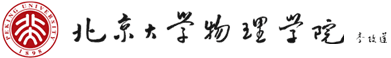
\includegraphics[width=.75\linewidth]{../PKUPhy}}
	}
	% Separator
	\newcommand{\newparagraph}{\pagebreak[3]\noindent%
		\hfil
		~\raisebox{-4pt}[10pt][10pt]{\decofourright~~~~~~~~\decofourleft}~ %
		\par
	}
%	% Background % Use when necessary
%	\usepackage{background} %Waterstamp package
%	\SetBgContents{...的实验报告} %Waterstamp to prevent copying
%	\SetBgScale{5} %Waterstamp setting
	% Essay format
	\renewcommand\appendixname{附录}
	\renewcommand\abstractname{}
	\renewcommand\tablename{表}
	\renewcommand\figurename{图}
	\renewcommand\refname{参考文献}
	\renewcommand\contentsname{目录}
	\makeatletter
	\def\@pacs@name{\songti\zihao{-4}{\bf PACS码:}}
	\def\@keys@name{\songti\zihao{-4}{\bf 关键词:}}
	\def\Dated@name{日期:}
	\def\Received@name{\zihao{-5}{接收} }
	\def\Revised@name{\zihao{-5}{修订} }
	\def\Accepted@name{\zihao{-5}{采纳} }
	\def\Published@name{\zihao{-5}{发表} }
	\makeatother
	\linespread{1.5}
	\renewcommand{\labelenumi}{\alph{enumi}.}
	\leftmargini=20mm
	\newcommand{\supercite}[1]{\textsuperscript{\,%
		[\citenum{#1}]}}
	\let\fancycite\cite
	\renewcommand{\cite}[1]{\textup{\fancycite{#1}}}

%Miscellaneous
%	\newcommand{\tabindent}{\hspace{2em}}
%FourierTransform
	\newcommand{\fourierf}{\mathscr F}
\begin{document}
%Basic Data
	\title{%
	\texstringonly{\hfil\\[2\baselineskip]}
	\sf\LARGE%
		He-Ne激光器模式分析%
	\texstringonly{\vspace{3ex}}}
	\author{\fangsong\large%
		吴熙楠%
	\vspace{2mm}}
	\affiliation{\it%
		北京大学物理学院~~学号:\normalfont 1900011413\,}
	\date{\today}
	\keywords{He-Ne激光器, 共焦球面扫描干涉仪, 横纵模}
	\email{xinanwu@pku.edu.cn;}
	
\begin{abstract}
\vspace{10mm}
\begin{spacing}{1.5}\normalsize
\setlength{\parskip}{.3\baselineskip}
%	200—300字,
%	说明用什么方法做了什么事,
%	由此得到什么结果和结论,
%	有何意义. 
%	不用缩略词,不用第一人称.
%	
本实验利用共焦球面扫描干涉仪测量了He-Ne激光器的模式的频谱分布, 并得到了纵模横模频率间隔, 也得到扫描干涉仪的精细常数, 并判断出了示波器上频率增加的方向. 本实验对于理解激光器的不同横纵模具有较大意义, 并提供了测量激光模式间隔的方法.
\end{spacing}
\end{abstract}
\clearpage
\maketitle
\thispagestyle{titlepagestyle}
%
%	\item 课程实验报告应假定读者既不是已知全部实验细节的指导教师,也不是缺少专业知识的公众,而是同领域的实验研究者,或审稿人. 不能要求读者要在读过课程讲义后才能读懂课程实验报告.
%	\item 公式、图和表要分别用阿拉伯数字编列序号. 公式和图表要达到可发表的质量.
%	\item 凡不是自己独立思考得到的内容都应该引参考文献. 不能大段引用同一参考文献. 对复杂问题,应该优先考虑引用参考文献得到结果. 对简单一些的问题才鼓励独立思考.
%	\item 较长的推导和说明可以作为附件提交,不占用报告篇幅.
%	\item 思考题不是报告的组成部分. 应另起一页附在报告的最后.

\newpage
\section{引言}
%	研究论文引言一般包含以下内容:
%	(1)所研究领域背景和现状;
%	(2)有待研究的问题;
%	(3)本研究的目的、主要内容和结果;
%	(4)结果的意义.\par
%	在写实验报告的引言时,同学可以假想自己是第一个做类似研究的人.\par
%	引言一定要切合报告正文,不能漫无目的地介绍背景. 要快速地将读者引导到报告主题上,并作较深入的讨论.\par
%	引言篇幅可以在较大范围内变化,但最长不应超过报告文字篇幅的1/3.\par
%	引言撰写可以参考实验讲义,可以复述,但不能复制讲义上的任何一句话.\par
%%%%%%%%%%%%%%%%%%%%%%%%%%%%%%
激光以其单色性好, 相干性好而著称. 本实验以He-Ne激光器作为研究对象, 利用共焦球面扫描干涉仪得到激光器中不同的激光模式的频率, 分析其特征, 以加深对于激光的理解.
\section{理论}
\subsection{激光的横模纵模}
本实验中采用的是He-Ne激光器, 所用的腔为简单的两个反射镜组成的腔. 光在谐振腔中往返一周的光程差是波长整数倍的时候会被放大, 即$2L=q\lambda_q$(已取介质折射率约为1的近似). 不同q对应于不同的纵模, 因而相邻纵模的频率差为$\Delta \nu_(\Delta q=1)=\dfrac{c}{2L}$ . 不过一个模式不仅对应于纵向的一种稳定的电磁场的分布, 也对应于横向的电磁场的一种稳定分布, 称为横模. 不同的横模的电磁场场强在x或y方向的零点数目不一样. 由理论可知相邻横模之间的频率差为$\Delta \nu_{\Delta m+\Delta n=1}=\Delta \nu_{\Delta q=1} {\dfrac{1}{\pi}  arccos⁡[\sqrt{(1-\dfrac{L}{R_1})(1-\dfrac{L}{R_2})}]}$ , 其中$R_1,R_2$为谐振腔的两个反射镜的曲率半径, 由此可以计算出理论上所用的He-Ne激光器的横纵模频率间隔. 
\subsection{共焦球面扫描干涉仪}
	\begin{figure}[!h]
	\centering
	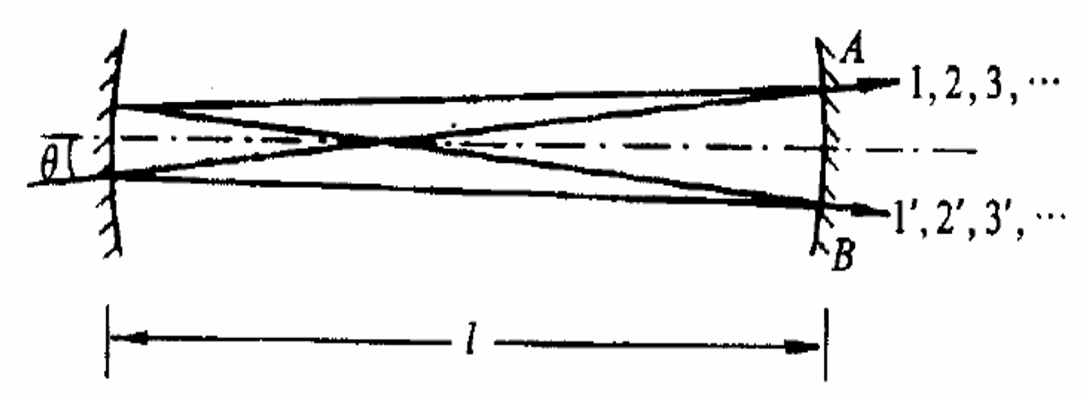
\includegraphics[width=.8\linewidth]{img/1.png}
	\caption[共焦球面扫描干涉仪内部光路图]{共焦球面扫描干涉仪内部光路图}\vspace{1ex}
	\end{figure}
扫描干涉仪的具体原理:近光轴方向射入干涉仪的激光在两块曲率半径与腔长相等的反射镜之间传播的时候走过的路程为如图所示的X形(可以通过球面反射镜的成像公式推得), 因而光走4l是一个周期, 每个周期也都会有光从镜面透射而出; 若4l是某个波长$\lambda_a$的整数倍, 则波长为$\lambda_a$将产生相干极大透射, 而其他波长则会抵消. 若外加电压使腔长发生微小变化, 相应的产生极大透射的波长也会发生变化, 并且波长和腔长一一对应. 因而用一定幅度的交流电压来改变腔长就能使得激光器不同频率的模式一次产生相干极大透射, 从而实现频谱的扫描. 但扫描干涉仪有重序现象, 即在$4l=k\lambda_b=(k+1)\lambda_a$的时候分辨不出这两个波长, 因而测量的频谱是有一定范围的. 经推导可知扫描干涉仪所能扫出的不重序的最大频率差, 即自由光谱范围, 为$\Delta\nu_{S.R.}=\dfrac{c}{4l}$ ; 实验中要保证自由光谱范围大于所测量的光谱范围. 扫描干涉仪的精细常数表征干涉仪的分辨本领, 实验的角度来说, 精细常数的定义为$F=\dfrac{\delta\lambda_{S.R.}}{\delta\lambda}$ ,其中$\delta\lambda$即为干涉仪所能分辨出的最小波长差, 实验中可以用一个模的半宽来代替.
\section{实验装置}
%	在此部分需要将实验条件交待清楚到别人能重复你的实验结果的程度. 此外,还需表明你已尽了最大努力来提高实验精度和结果的可靠性. 简单的不确定度估计可以在此节给出,复杂一些的可以放到分析讨论部分.\par
%	实验条件不仅是指直接影响实验结果的实验参量,而且还包括影响实验质量和可靠性的因素,如室温、空气湿度、基真空、原材料纯度等.\par
%	作为教学实验报告,此节写详细一点没有坏处.\par
%	成段有叙述,必要才分节。
%%%%%%%%%%%%%%%%%%%%%%%%%%%%%%
	\begin{figure}[!h]
	\centering
	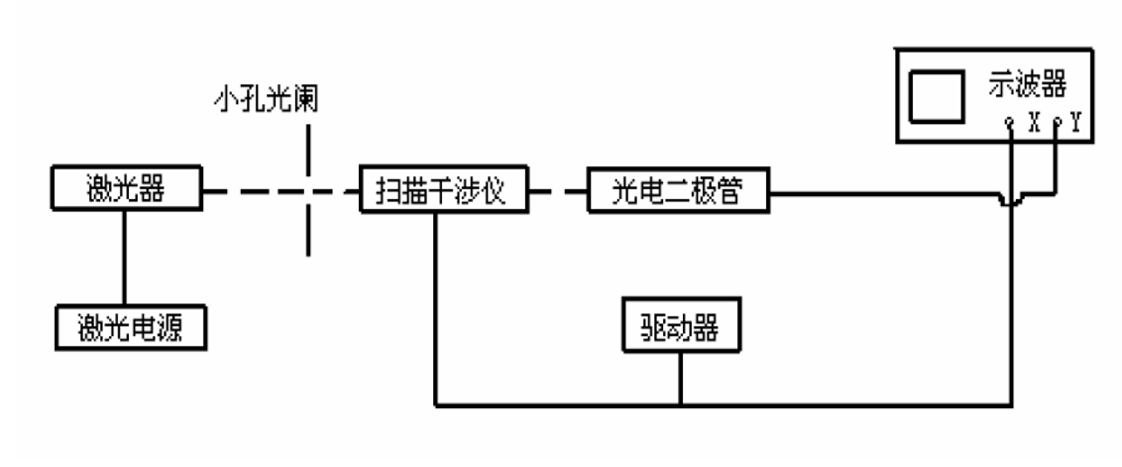
\includegraphics[width=.8\linewidth]{img/2.png}
	\caption[实验装置示意图]{实验装置示意图}\vspace{1ex}
	\end{figure}
\par 实验中是采用共焦球面扫描干涉仪来获得激光束中的不同的频率成分. 激光束经过小孔光阑限制其宽度之后经过扫描干涉仪, 之后的信号经过光点二极管进行放大, 然后成像与示波器上.驱动器中加入锯齿波使得扫描干涉仪可以扫描得到信号, 同时其也作为X轴信号输入示波器. 在X-Y模式下即可在示波器上看到频谱图.
\par 实验中在光路中加上小孔光阑之后调节扫描干涉仪, 信号放大器与激光器共轴, 小孔光阑在调节好共轴之后即可撤去. 本次实验中在调节共轴之后又小幅调节使得信噪比接近于最大. 实验在室温下进行.
\section{结果与分析}
%	实验结果应尽量以图表的形式给出. 每一个图表都应该是完整的,即阅读图表时可以不必依赖正文.\par
%	依自己意愿,实验结果和对结果的分析讨论既可分为两节也可合在一节.\par
%	\begin{table}[h]
%	\caption{元件恒流大小,为什么要左对齐呢?奇怪。}
%	\small
%	\begin{tabularx}{.6\linewidth}{C{.3} C{1}}
%	\toprule
%	\midrule
%		元件\footnote{%
%			注释一个看看%
%		} & 恒流大小\footnote{%
%			再开一个!哈哈
%		} \\
%	\midrule
%		Pt  &
%			$\SI{1.00005}{\mA}
%				= \SI{100.005}{\mV} / \SI{100}{\ohm} $ \\
%	\midrule
%	\bottomrule
%	\end{tabularx}
%	\label{tab:ExTab}
%	\end{table}
%	
%	每个图一般包含:图名、轴名、轴、刻度、标尺、数据点、曲线、图例、标注和图注等部分. 应尽量让读者不看正文就能基本理解图的含意.\par
%	逐点测量得到的函数关系要同时用表格和图给出. 需要作比较的多条曲线要画在同一图上.\par
%	为避免读者在图表和正文间反复跳跃阅读,在正文中也要对图表作必要的说明.\par
%	
%	对于预料之外的实验结果,必须首先小心证明其可靠性.读者只有在相信你的实验结果时才愿意花时间看你的分析.\par
%	必须用文字归纳整理出正式的实验结果或结论.可信的实验结果是课程报告最重要的内容.作为一个实验物理工作者,分析解释出错并不丢脸,实验结果不被采信则是致命的.\par
%	教学实验的结论往往是预先知道的. 所以,教师更关心的是你的说理过程. 一般说来,单由课内实验的结果不足以能得到明确的结论. 此时,你可以引用他人的研究结果来帮助帮助自己的论证,但必须注明出处. \par
%	确实不能得到明确结论时,可以给出几种可能结论并指出可以再做哪些实验来帮助作进一步的判断.\par
%	总之,分析讨论部分要做到: 论据要valid,论证要reasonable,结论要convincing.\par
%%%%%%%%%%%%%%%%%%%%%%%%%%%%%%

\section{结论}
%	首先要给出实验结果,然后再给出由实验结果分析得到的结果和结论.此部分给出的内容要比摘要中的全面,用词要更准确.\par
本实验利用共焦球面扫描干涉仪测量了两个腔长不同的He-Ne激光器的模式在频谱上的分布, 并得到了各自的纵模横模频率间隔, 将其余理论值比较, 差别在误差范围内; 也得到扫描干涉仪的精细常数(约118), 并判断出了示波器上频率增加的方向为向右. 本实验对于理解激光器的不同横纵模具有较大意义, 并提供了测量激光模式间隔的方法.
\section{思考题}
1.根据什么确定干涉仪扫出的干涉序的个数?
\par 答:根据频谱图的周期性, 可以确定每个干涉序, 从而可以得知干涉序的个数.

2.辨认不同的纵模和横模的依据.
\par 答:在本实验所用的激光器的相邻横模间隔较小, 因而间隔较小的为同一纵模不同横模的模式, 间隔较大的为不同纵模的模式.

3.观测时, 为何要先确定示波器上被扫出的干涉序的数目, 又何好处?
\par 答: 这样可以选出同一个干涉序进行测量, 然后由干涉序对应的示波器横轴的格数来标定每格对应的频率差.

4.本实验方法的优缺点.
\par 答:缺点: 噪声较大, 部分纵模随时间波动较明显, 使得测量有一定的困难; 使用示波器面板肉眼读数, 误差比用数字方法读数要大. 
优点: 扫描干涉仪扫描较准确, 得到多条激光模式.

5.在示波器的不同位置, 纵模频率间隔有所差异的原因是什么? 如何提高测量的准确度?
\par 答:控制扫描干涉仪腔长的压电陶瓷的长度变化量对所加电压的响应可能偏离线性, 导致测量有一定误差. 
提高测量精度方法: 一是可以选用线性程度更好的压电陶瓷; 二是可以改变示波器横轴放大倍数使得测量更加准确.

\section{致谢}
%	此部分感谢同组人...和对实验和报告有帮助的人.
	感谢我的合作伙伴杨轩同学,他的工作是不可或缺的;感谢耐心的胡小永指导老师对我们的巨大帮助。
\begin{thebibliography}{99}
	\addcontentsline{toc}{section}{参考文献}
	\bibitem{ref1}北京大学物理学院光学所, 激光实验, 第二版, 北京: 北京大学物理学院, 2023.
\end{thebibliography}
\clearpage
\end{document}
